%-------------------------------------------------------------------------------
\documentclass[twocolumn]{article}

%-------------------------------------------------------------------------------
% Packages
\usepackage[portuguese]{babel}
\usepackage{environ}
\usepackage[margin=2cm]{geometry}
\usepackage{graphicx}
\usepackage{hyperref}
\usepackage{minted}
\usepackage{xcolor}

%-------------------------------------------------------------------------------
% User-commands
\newcommand{\todo}[1]{{\color{red}{#1}}}

\NewEnviron{superframe}{%
    \begin{center}
        \fbox{\setlength{\fboxsep}{1em}\fbox{\parbox{5.5in}{%
            \BODY{}
        }}}
    \end{center}
}

\newmintedfile[textfile]{text}{autogobble, breaklines}

%-------------------------------------------------------------------------------
% Project configs
\title{Relatório de I.A.: Sistemas Fuzzy (Trabalho 4)}
\author{Cauê Baasch de Souza \\
        João Paulo Taylor Ienczak Zanette}
\date{\today}

%-------------------------------------------------------------------------------
\begin{document}
    \maketitle{}

    \todo{%
        TO-DO\@:
        \begin{itemize}
            \item Descrever tutorial breve de Fuzzy;
            \item Entradas;
            \item Conjuntos Fuzzy;
            \item Regras;
            \item Método de defuzzificação;
            \item Dificuldades encontradas e como foram superadas.
        \end{itemize}
    }

    \section{Introdução: O ``Fuzzy Truck''}

    Em um curso de Computação, é comum que se aprenda inicialmente a resolver
    problemas utilizando Lógica Proposicional, em que se julgam diferentes
    assertivas como ``verdadeiras'' ou ``falsas''. Tomando um exemplo simplista
    de previsão do tempo, pode-se partir das preposições:

    \begin{itemize}
        \item $h$: fez calor (\textit{``hot''});
        \item $c$: está nublado (\textit{``cloudy''});
        \item $r$: irá chover (\textit{``rain''}).
    \end{itemize}

    A partir delas, é possível estabelecer a relação ``se fez calor e está
        nublado, então irá chover'', conforme descrito na Equação~\ref{will-rain}:

    \begin{equation}
        \label{will-rain}
        h \land c \rightarrow r
    \end{equation}

    Porém, é de se concordar que fazer calor e estar nublado não são tão
    simples de se definir apenas com ``verdadeiro'' e ``falso'', mas sim como
    ``o quão quente'' e ``o quão nublado''. Esse é o ponto que Lógica Fuzzy
    ataca: a possibilidade de atribuir graus de verdade às assertivas dadas.
    Assim, é possível mapear que, dada a temperatura ao longo do dia (pode-se
    considerar, por exemplo, o ponto mais alto da temperatura), ela esteja mais
    próxima de fria quanto mais próxima de 0ºC, ou de quente quanto mais
    próxima de 40ºC, ou amena quanto mais próxima de 20ºC. Esses diferentes
    intervalos com seus respectivos significados são chamados de ``Conjuntos
    Fuzzy''. A Figura~\ref{time-fuzzifiers} descreve graficamente tais
    conjuntos para o problema de previsão do tempo, adicionando os conjuntos
    ``sem nuvens'', ``esparso'' e ``nublado'' para densidade de nuvens
    (respectivamente, ``\textit{no\_clouds}'', ``\textit{sparse}'' e
    ``\textit{cloudy}'') e ``não'', ``um pouco'' e ``muito'' para se irá chover
    (respectivamente, ``\textit{no}'', ``\textit{a\_little}'' e
    ``\textit{a\_lot}'').

    \begin{figure}[h!]
        \centering
        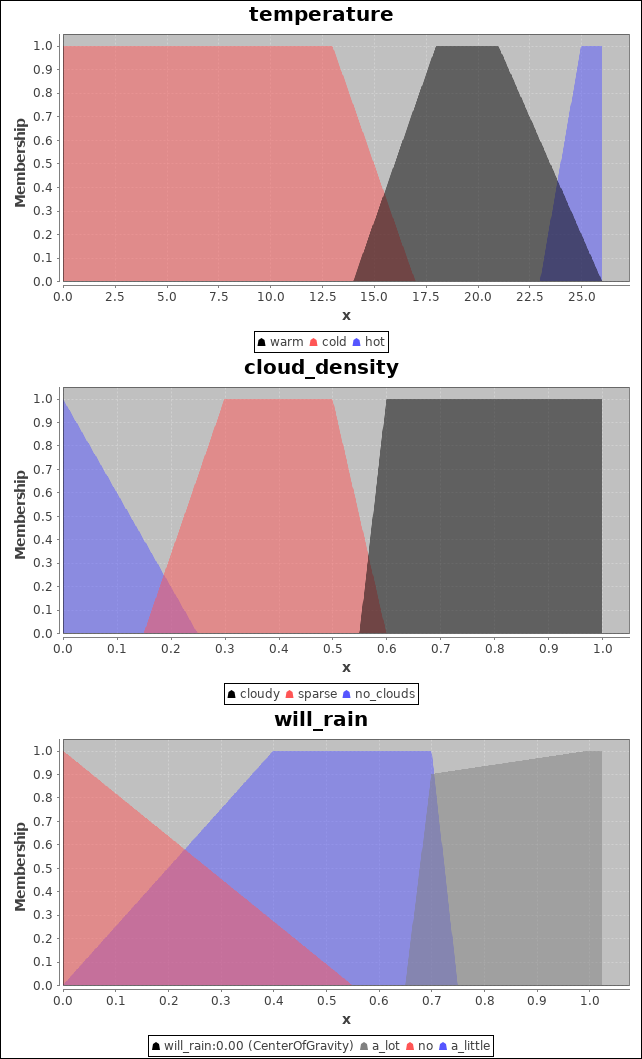
\includegraphics[keepaspectratio,width=0.45\textwidth]{img/time-fuzzifiers}
        \caption{Conjuntos Fuzzy para dados de entrada (temperatura e densidade
        de nuvens) e saída (``irá chover''), respectivamente, de um sistema
        Fuzzy para previsão do tempo.\label{time-fuzzifiers}}
    \end{figure}

    Para se inferir o resultado (no exemplo: se irá chover), utilizam-se regras
    descritas com lógica proposicional que indicam qual a tendência de um
    resultado conforme as condições de cada regra. Para o exemplo em questão,
    poderiam-se utilizar três regras:

    \begin{enumerate}
        \item Temperatura é amena $\land$ está nublado $\rightarrow$ irá chover
            um pouco;
        \item Temperatura é quente $\land$ está nublado $\rightarrow$ irá
            chover muito;
        \item Temperatura é quente $\land$ núvens estão esparsas $\rightarrow$
            irá chover um pouco.
    \end{enumerate}

    E, então, considera-se que em qualquer caso distinto desses não irá chover.
    Aplicando uma função em cima dos parâmetros de temperatura e densidade de
    núvens, pode-se inferir então qual regra é mais aplicável a cada caso (ou o
    padrão, caso nenhuma se aplique o suficiente). Esta etapa é chamada de
    Defuzzificação.

    Como aplicação prática, se leva em conta o problema do ``Fuzzy Truck''.
    Nele, é necessário definir parâmetros, saídas e regras para fazer um
    caminhão estacionar em uma doca de ré, considerando um espaço 2D sem
    obstáculos. Como restrições do problema, o caminhão possui velocidade
    constante (com exceção de que ele para quando está suficientemente próximo
    do espaço que delimita a vaga) e suas únicas ações possíveis são: girar o
    volante para a esquerda (indicado pelo valor -1), manter a direção atual do
    caminhão (valor 0) e girar o volante para a direita (valor 1).

    \section{Resolvendo o problema do ``Fuzzy Truck''}

    \subsection{Entradas utilizadas e Conjuntos Fuzzy}

    Foram utilizadas três entradas simples: as coordenadas $x$ e $y$ e o ângulo
    do caminhão (em graus). Os conjuntos fuzzy foram definidos (

    \subsection{Regras utilizadas}

    \subsection{Defuzzificação}

    \section{Conclusões e considerações}

    \bibliographystyle{unsrt}
    \bibliography{refs}
    \nocite{*}
\end{document}
